\documentclass[journal,12pt,twocolumn]{IEEEtran}
\usepackage{setspace}
\usepackage{gensymb}
\usepackage{caption}
%\usepackage{multirow}
%\usepackage{multicolumn}
%\usepackage{subcaption}
%\doublespacing
\singlespacing
\usepackage{csvsimple}
\usepackage{amsmath}
\usepackage{multicol}
%\usepackage{enumerate}
\usepackage{amssymb}
%\usepackage{graphicx}
\usepackage{newfloat}
%\usepackage{syntax}
\usepackage{listings}
\usepackage{iithtlc}
\usepackage{color}
\usepackage{tikz}
\usetikzlibrary{shapes,arrows}



%\usepackage{graphicx}
%\usepackage{amssymb}
%\usepackage{relsize}
%\usepackage[cmex10]{amsmath}
%\usepackage{mathtools}
%\usepackage{amsthm}
%\interdisplaylinepenalty=2500
%\savesymbol{iint}
%\usepackage{txfonts}
%\restoresymbol{TXF}{iint}
%\usepackage{wasysym}
\usepackage{amsthm}
\usepackage{mathrsfs}
\usepackage{txfonts}
\usepackage{stfloats}
\usepackage{cite}
\usepackage{cases}
\usepackage{mathtools}
\usepackage{caption}
\usepackage{enumerate}	
\usepackage{enumitem}
\usepackage{amsmath}
%\usepackage{xtab}
\usepackage{longtable}
\usepackage{multirow}
%\usepackage{algorithm}
%\usepackage{algpseudocode}
\usepackage{enumitem}
\usepackage{mathtools}
\usepackage{hyperref}
%\usepackage[framemethod=tikz]{mdframed}
\usepackage{listings}
    %\usepackage[latin1]{inputenc}                                 %%
    \usepackage{color}                                            %%
    \usepackage{array}                                            %%
    \usepackage{longtable}                                        %%
    \usepackage{calc}                                             %%
    \usepackage{multirow}                                         %%
    \usepackage{hhline}                                           %%
    \usepackage{ifthen}                                           %%
  %optionally (for landscape tables embedded in another document): %%
    \usepackage{lscape}     


\usepackage{url}
\def\UrlBreaks{\do\/\do-}


%\usepackage{stmaryrd}


%\usepackage{wasysym}
%\newcounter{MYtempeqncnt}
\DeclareMathOperator*{\Res}{Res}
%\renewcommand{\baselinestretch}{2}
\renewcommand\thesection{\arabic{section}}
\renewcommand\thesubsection{\thesection.\arabic{subsection}}
\renewcommand\thesubsubsection{\thesubsection.\arabic{subsubsection}}

\renewcommand\thesectiondis{\arabic{section}}
\renewcommand\thesubsectiondis{\thesectiondis.\arabic{subsection}}
\renewcommand\thesubsubsectiondis{\thesubsectiondis.\arabic{subsubsection}}

% correct bad hyphenation here
\hyphenation{op-tical net-works semi-conduc-tor}

%\lstset{
%language=C,
%frame=single, 
%breaklines=true
%}

%\lstset{
	%%basicstyle=\small\ttfamily\bfseries,
	%%numberstyle=\small\ttfamily,
	%language=Octave,
	%backgroundcolor=\color{white},
	%%frame=single,
	%%keywordstyle=\bfseries,
	%%breaklines=true,
	%%showstringspaces=false,
	%%xleftmargin=-10mm,
	%%aboveskip=-1mm,
	%%belowskip=0mm
%}

%\surroundwithmdframed[width=\columnwidth]{lstlisting}
\def\inputGnumericTable{}                                 %%
\lstset{
%language=C,
frame=single, 
breaklines=true,
columns=fullflexible
}
 

\begin{document}
%
\tikzstyle{block} = [rectangle, draw,
    text width=3em, text centered, minimum height=3em]
\tikzstyle{sum} = [draw, circle, node distance=3cm]
\tikzstyle{input} = [coordinate]
\tikzstyle{output} = [coordinate]
\tikzstyle{pinstyle} = [pin edge={to-,thin,black}]

\theoremstyle{definition}
\newtheorem{theorem}{Theorem}[section]
\newtheorem{problem}{Problem}
\newtheorem{proposition}{Proposition}[section]
\newtheorem{lemma}{Lemma}[section]
\newtheorem{corollary}[theorem]{Corollary}
\newtheorem{example}{Example}[section]
\newtheorem{definition}{Definition}[section]
%\newtheorem{algorithm}{Algorithm}[section]
%\newtheorem{cor}{Corollary}
\newcommand{\BEQA}{\begin{eqnarray}}
\newcommand{\EEQA}{\end{eqnarray}}
\newcommand{\define}{\stackrel{\triangle}{=}}

\bibliographystyle{IEEEtran}
%\bibliographystyle{ieeetr}

\providecommand{\nCr}[2]{\,^{#1}C_{#2}} % nCr
\providecommand{\nPr}[2]{\,^{#1}P_{#2}} % nPr
\providecommand{\mbf}{\mathbf}
\providecommand{\pr}[1]{\ensuremath{\Pr\left(#1\right)}}
\providecommand{\qfunc}[1]{\ensuremath{Q\left(#1\right)}}
\providecommand{\sbrak}[1]{\ensuremath{{}\left[#1\right]}}
\providecommand{\lsbrak}[1]{\ensuremath{{}\left[#1\right.}}
\providecommand{\rsbrak}[1]{\ensuremath{{}\left.#1\right]}}
\providecommand{\brak}[1]{\ensuremath{\left(#1\right)}}
\providecommand{\lbrak}[1]{\ensuremath{\left(#1\right.}}
\providecommand{\rbrak}[1]{\ensuremath{\left.#1\right)}}
\providecommand{\cbrak}[1]{\ensuremath{\left\{#1\right\}}}
\providecommand{\lcbrak}[1]{\ensuremath{\left\{#1\right.}}
\providecommand{\rcbrak}[1]{\ensuremath{\left.#1\right\}}}
\theoremstyle{remark}
\newtheorem{rem}{Remark}
\newcommand{\sgn}{\mathop{\mathrm{sgn}}}
\providecommand{\abs}[1]{\left\vert#1\right\vert}
\providecommand{\res}[1]{\Res\displaylimits_{#1}} 
\providecommand{\norm}[1]{\left\Vert#1\right\Vert}
\providecommand{\mtx}[1]{\mathbf{#1}}
\providecommand{\mean}[1]{E\left[ #1 \right]}
\providecommand{\fourier}{\overset{\mathcal{F}}{ \rightleftharpoons}}
%\providecommand{\hilbert}{\overset{\mathcal{H}}{ \rightleftharpoons}}
\providecommand{\system}{\overset{\mathcal{H}}{ \longleftrightarrow}}
	%\newcommand{\solution}[2]{\textbf{Solution:}{#1}}
\newcommand{\solution}{\noindent \textbf{Solution: }}
\newcommand{\myvec}[1]{\ensuremath{\begin{pmatrix}#1\end{pmatrix}}}
\providecommand{\dec}[2]{\ensuremath{\overset{#1}{\underset{#2}{\gtrless}}}}
\DeclarePairedDelimiter{\ceil}{\lceil}{\rceil}
%\numberwithin{equation}{subsection}
%\numberwithin{equation}{section}
%\numberwithin{problem}{subsection}
%\numberwithin{definition}{subsection}
\makeatletter
\@addtoreset{figure}{section}
\makeatother

\let\StandardTheFigure\thefigure
%\renewcommand{\thefigure}{\theproblem.\arabic{figure}}
\renewcommand{\thefigure}{\thesection}


%\numberwithin{figure}{subsection}

%\numberwithin{equation}{subsection}
%\numberwithin{equation}{section}
%\numberwithin{equation}{problem}
%\numberwithin{problem}{subsection}
\numberwithin{problem}{section}
%%\numberwithin{definition}{subsection}
%\makeatletter
%\@addtoreset{figure}{problem}
%\makeatother
\makeatletter
\@addtoreset{table}{section}
\makeatother

\let\StandardTheFigure\thefigure
\let\StandardTheTable\thetable
\let\vec\mathbf
%%\renewcommand{\thefigure}{\theproblem.\arabic{figure}}
%\renewcommand{\thefigure}{\theproblem}

%%\numberwithin{figure}{section}

%%\numberwithin{figure}{subsection}



\def\putbox#1#2#3{\makebox[0in][l]{\makebox[#1][l]{}\raisebox{\baselineskip}[0in][0in]{\raisebox{#2}[0in][0in]{#3}}}}
     \def\rightbox#1{\makebox[0in][r]{#1}}
     \def\centbox#1{\makebox[0in]{#1}}
     \def\topbox#1{\raisebox{-\baselineskip}[0in][0in]{#1}}
     \def\midbox#1{\raisebox{-0.5\baselineskip}[0in][0in]{#1}}

\vspace{3cm}

\title{ 
	\logo{
JEE Problems in Calculus
	}
}

%\author{ G V V Sharma$^{*}$% <-this % stops a space
%	\thanks{*The author is with the Department
%		of Electrical Engineering, Indian Institute of Technology, Hyderabad
%		502285 India e-mail:  gadepall@iith.ac.in. All content in this manual is released under GNU GPL.  Free and open source.}
	
%}	

\maketitle

%\tableofcontents

\bigskip

\renewcommand{\thefigure}{\theenumi}
\renewcommand{\thetable}{\theenumi}


\begin{abstract}
	A  collection of problems from JEE papers related to calculus are available in this document.  Verify your soluions using  numerical techniques for integration and differentiation.
\end{abstract}
\section{Calculus: Integration}
\begin{enumerate}[label=\thesection.\arabic*
,ref=\thesection.\theenumi]

\item Sketch the region 
\begin{align}
\myvec{x \\ y}: xy \le 8, 1\le y \le x^2
\end{align}
%
\item Find the area of the region.
\\ 
\solution The intersection of $y = 1, y = x^2$ is
\begin{align}
\vec{A} = \myvec{1 \\ 1}
\end{align}
The intersection of $y = 1, xy = 8$ is
\begin{align}
\vec{B} = \myvec{8 \\ 1}
\end{align}
%%
The intersection of $y = x^2, xy = 8$ is
\begin{align}
\vec{C} = \myvec{2 \\ 4}
\end{align}
%
The desired region is enclosed by the vertices $\vec{A},\vec{B}$ and 
$\vec{C}$
\begin{figure}
\centering
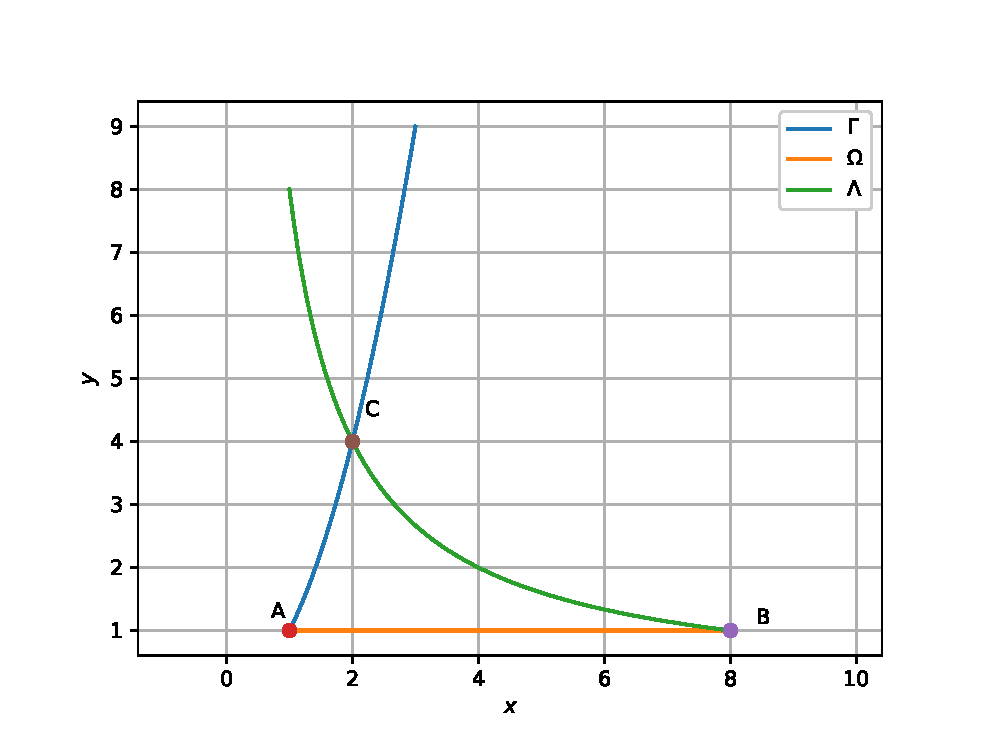
\includegraphics[width=\columnwidth]{./figs/2019_4.eps}
\caption{}
\label{fig:2019_4}
\end{figure}
%
Thus, the area is obtained as
\begin{align}
\int_{1}^{2}x^2\,dx + \int_{2}^{8}\frac{8}{x}\,dx
&= \sbrak{\frac{x^3}{3}}_{1}^{2}+8 \sbrak{\ln x}_{2}^{8} - 7
\\
&= 16 \ln 2 - \frac{14}{3}
\end{align}
\end{enumerate}
\section{Calculus: Differentiation}
Let 
{\small
\begin{align}
f(x) = 
\begin{cases}
x^5+5x^4+10x^3+10x^2+3x+1 & x < 0
\\
x^2-x+1 & 0 \le  x < 1
\\
\frac{2}{3}x^3-4x^2+7x-\frac{8}{3} & 1 \le x < 3
\\
\brak{x-2}\ln \brak{x-2}-x + \frac{10}{3} & x \ge 3
\end{cases}
\end{align}
}
\begin{enumerate}[label=\thesection.\arabic*
,ref=\thesection.\theenumi]
\item Is $f$ increasing in $\brak{-\infty, 0}$?	
\\
\solution 
\begin{align}
f^{\prime}(x) = 5x^4+20x^3+30x^2+20x+3 \quad  x < 0 &
\nonumber \\
\implies f^{\prime}(-1) = 5-20+30-20+3 =-2 < 0 &
\end{align}
%
Hence $f^{\prime}(x)$ is non-increasing.

\item Does $f^{\prime}$ have a local maximum at $x = 1$?
\\
\solution 
\begin{align}
\label{eq:cont_diff}
f^{\prime}(x)=
\begin{cases}
  2x-1 > 0, &  \frac{1}{2} < x < 1,
\\
2\brak{x-2}^2 -1 < 0 & 1 \le x < 3
\end{cases}
\end{align}
Hence, $f$ is increasing in $\brak{\frac{1}{2},1}$ and decreasing between $\brak{1, 3} \implies f$ has a local maximum at $x=1$
\item Show that $f^{\prime}$ is differentiable at $x = 1$.
\\
\solution Since
\begin{align}
f^{\prime}(1-)=
f^{\prime}(1)=1,
\end{align}
$f$ is differentiable at $x = 1$.
\item Is $f$ onto?
\item Sketch $f(x)$ in Python to verify your answeres.

\end{enumerate}

\section{Calculus: Differential Equations}
$\Gamma$ is a curve in the first qudrant and 
\begin{align}
\vec{R} = \myvec{1 \\ 0}
\end{align}
%
lies on it.  The tangent to $\Gamma$ at $\vec{P}$ intersects the $y-$axis at $\vec{Y}_P$. The line segment $PY_P = 1$. 
%
\begin{enumerate}[label=\thesection.\arabic*
,ref=\thesection.\theenumi]
\item Find the differential equation of $\Gamma$.
\\
\solution Let 
\begin{align}
\vec{P}=\myvec{x \\ y},
\vec{Y}_P=\myvec{0 \\ c}.
\end{align}
%
Then using the equation of a line, 
\begin{align}
\vec{Y}_P=\vec{P} + \lambda \vec{m},
\end{align}
%
where 
\begin{align}
\vec{m}=\myvec{1\\ y^{\prime}}.
\end{align}
%
Thus, 
\begin{align}
\myvec{0 \\ c}&=\myvec{x \\ y} + \lambda \myvec{1\\ y^{\prime}}
\\
\implies \lambda &= -x.
\end{align}
\begin{align}
\because PY_P =  \norm{\vec{P}-\vec{Y}_P} &= \abs{\lambda} \norm{\vec{m}} = 1,
\\
x^2\brak{1 + \brak{y^{\prime}}^2} &= 1
\\
\implies xy^{\prime}  \pm \sqrt{1-x^2} &= 0
\label{eq:diffeq}
\end{align}
%
\item Find the equation of $\Gamma$.
\\
\solution From \eqref{eq:diffeq},
\begin{align}
dy &=   \pm \frac{\sqrt{1-x^2}}{ x}\,dx
\\
\implies \int \, dy &=   \pm \int\frac{\sqrt{1-x^2}}{ x}\,dx
%\label{eq:diffeq}
\end{align}
%
Letting 
\begin{align}
z = \sqrt{1-x^2},
dz &= -\frac{x}{\sqrt{1-x^2}}\, dx
\nonumber \\
\implies \int\frac{\sqrt{1-x^2}}{ x}\,dx &= -\int\frac{z^2}{ 1-z^2}\,dz
\nonumber \\
 &= \int\,dz-\int\frac{1}{ 1-z^2}\,dz
\nonumber \\
 &= z + \frac{1}{2}\ln \frac{1-z}{1+z} + C
\end{align}
Thus, 
\begin{align}
y = \pm \brak{\sqrt{1-x^2} + \frac{1}{2}\ln \frac{1-\sqrt{1-x^2}}{1+\sqrt{1-x^2}}} 
\end{align}
since $C=0$ after substituting $x=0, y = 1$.
\item Verify your result through a python sketch.
\end{enumerate}
\section{Calculus: Definite Integral}
\begin{enumerate}[label=\thesection.\arabic*
,ref=\thesection.\theenumi]

\item If 
\begin{align}
\label{eq:17}
I = \frac{2}{\pi}\int_{-\frac{\pi}{4}}^{\frac{\pi}{4}}\frac{dx}{\brak{1+e^{\sin x}}\brak{2-\cos 2x}},
\end{align}
find $27 I^2$.
\\
\solution Substituting $-x$ for $x$,
\begin{align}
\label{eq:17_neg}
I = \frac{2}{\pi}\int_{-\frac{\pi}{4}}^{\frac{\pi}{4}}\frac{dx}{\brak{1+e^{-\sin x}}\brak{2-\cos 2x}},
\end{align}
Adding \eqref{eq:17} and \eqref{eq:17_neg},
\begin{multline}
\label{eq:17_sum}
2I = \frac{2}{\pi}\int_{-\frac{\pi}{4}}^{\frac{\pi}{4}}\frac{dx}{\brak{2-\cos 2x}}\lsbrak{\frac{1}{\brak{1+e^{\sin x}}}}
\\
+\rsbrak{\frac{1}{\brak{1+e^{-\sin x}}}},
\end{multline}
%
which can be simplified to obtain
\begin{align}
I &= \frac{1}{\pi}\int_{-\frac{\pi}{4}}^{\frac{\pi}{4}}\frac{dx}{\brak{2-\cos 2x}}\frac{\brak{1+e^{\sin x}+1+e^{-\sin x}}}{\brak{1+e^{\sin x}+e^{-\sin x}+1}}
\nonumber \\
&= \frac{1}{\pi}\int_{-\frac{\pi}{4}}^{\frac{\pi}{4}}\frac{dx}{\brak{2-\cos 2x}}
\label{eq:17_simp}
\end{align}
%
Substituting
\begin{align}
\cos 2x = \frac{1-\tan^2 x}{1+\tan^2},
\end{align}
in \eqref{eq:17_simp} and simplifying,
\begin{align}
I&= \frac{1}{\pi}\int_{-\frac{\pi}{4}}^{\frac{\pi}{4}}\frac{\sec^2x}{\brak{1+3\tan^2 x}}\,dx
\nonumber \\
&= \frac{1}{\pi\sqrt{3}}\sbrak{\tan^{-1}\brak{\sqrt{3}\tan x}}_{-\frac{\pi}{4}}^{\frac{\pi}{4}}
\nonumber \\
&= \frac{2}{3\sqrt{3}}
\label{eq:17_sol}
\end{align}
resulting in 
\begin{align}
27I^2 = 4
\end{align}
\end{enumerate}
\section{Calculus: Limits}
Let
\begin{align}
\label{eq:qp2_4_p1}
P_1 = \lim_{h \to 0} \frac{f(h)-f(0)}{\sqrt{\abs{h}}}
\\
P_2 = \lim_{h \to 0} \frac{f(h)-f(0)}{h^2}
\label{eq:qp2_4_p2}
\end{align}
%
\begin{enumerate}[label=\thesection.\arabic*
,ref=\thesection.\theenumi]
\item Find $P_1$ for 
\begin{align}
\label{eq:qp2_4_absx}
f(x) =\abs{x}
\end{align}
\solution Substituting \eqref{eq:qp2_4_absx} in \eqref{eq:qp2_4_p1},
\begin{align}
\label{eq:qp2_4_absx_p1}
P_1 =\lim_{h\to 0}\frac{\abs{h}}{\sqrt{h}} = 0
\end{align}
\item Find $P_1$ for 
\begin{align}
\label{eq:qp2_4_x23}
f(x) =x^{\frac{2}{3}}
\end{align}
\solution Substituting \eqref{eq:qp2_4_x23} in \eqref{eq:qp2_4_p1},
\begin{align}
\label{eq:qp2_4_x23_p1}
P_1 =\lim_{h\to 0}\frac{h^{\frac{2}{3}}}{\sqrt{h}} = h^{\frac{1}{3}}=0
\end{align}
\item Find $P_2$ for 
\begin{align}
\label{eq:qp2_4_xabsx}
f(x) =x\abs{x}
\end{align}
\solution Substituting \eqref{eq:qp2_4_xabsx} in \eqref{eq:qp2_4_p2},
\begin{align}
\label{eq:qp2_4_xabsx_p2+}
\lim_{h\to 0+}\frac{h\abs{h}}{h^2} = 1 
\end{align}
and
\begin{align}
\label{eq:qp2_4_xabsx_p2-}
\lim_{h\to 0-}\frac{-h\abs{h}}{h^2} = -1
\\
\because \eqref{eq:qp2_4_xabsx_p2+}\ne \eqref{eq:qp2_4_xabsx_p2-},
\end{align}
$P_2$ does not exist.
\item Find $P_2$ for 
\begin{align}
\label{eq:qp2_4_sin}
f(x) =\sin x
\end{align}
\solution Substituting \eqref{eq:qp2_4_sin} in \eqref{eq:qp2_4_p2},
\begin{align}
\label{eq:qp2_4_sin}
\lim_{h\to 0+}\frac{\sin h}{h^2} = \infty
\end{align}
%
Hence $P_2$ does not exist.
\end{enumerate}
\section{Calculus: Maxima and Minima}
Let 
\begin{align}
\label{eq:qp2_5_max}
f(x) &= p(x)q(x), \quad x > 0, \text{ where}
\\
p(x) &= \sin \pi x
\\
q(x) &= \frac{1}{x^2}
%f^{\prime}(x) &= \frac{x^2\pi \cos \pi x - 2x\sin \pi x}{x^4} = 0
%\\
%\implies \tan x &= \frac{\pi x}{2}
\end{align}
%\begin{align}
%\label{eq:qp2_5_prob}
%f(x) = \frac{\sin \pi x}{x^2}, \quad x > 0
%\end{align}
\begin{enumerate}[label=\thesection.\arabic*
,ref=\thesection.\theenumi]
\item Show that $q(x)$ is monotonically decreasing.
\item Show that $p(x)$ is oscillatory. 
\item Find the regions where $f(x)$ is increasing and decreasing.
\\
\solution 
\begin{align}
\label{eq:qp2_5_fder}
\because
f^{\prime}(x) &= p(x)q^{\prime}(x)+p^{\prime}(x)q(x),
\\
q(x) &> 0, 
\\
q^{\prime}(x) & < 0, 
\end{align}
\begin{align}
\label{eq:qp2_5_fder+-}
f^{\prime}(x) 
\begin{cases}
< 0 & p(x) > 0 \text{ and } p^{\prime}(x) < 0
\\
 >  0 & p(x) < 0 \text{ and } p^{\prime}(x) > 0
\end{cases}
\end{align}
Table \ref{table:qp2_5} computes the desired regions based on \eqref{eq:qp2_5_fder+-}
\begin{table}[!h]
\centering
%\resizebox {0.5\columnwidth} {!} {
%%%%%%%%%%%%%%%%%%%%%%%%%%%%%%%%%%%%%%%%%%%%%%%%%%%%%%%%%%%%%%%%%%%%%%%
%%                                                                  %%
%%  This is the header of a LaTeX2e file exported from Gnumeric.    %%
%%                                                                  %%
%%  This file can be compiled as it stands or included in another   %%
%%  LaTeX document. The table is based on the longtable package so  %%
%%  the longtable options (headers, footers...) can be set in the   %%
%%  preamble section below (see PRAMBLE).                           %%
%%                                                                  %%
%%  To include the file in another, the following two lines must be %%
%%  in the including file:                                          %%
%%        \def\inputGnumericTable{}                                 %%
%%  at the beginning of the file and:                               %%
%%        \input{name-of-this-file.tex}                             %%
%%  where the table is to be placed. Note also that the including   %%
%%  file must use the following packages for the table to be        %%
%%  rendered correctly:                                             %%
%%    \usepackage[latin1]{inputenc}                                 %%
%%    \usepackage{color}                                            %%
%%    \usepackage{array}                                            %%
%%    \usepackage{longtable}                                        %%
%%    \usepackage{calc}                                             %%
%%    \usepackage{multirow}                                         %%
%%    \usepackage{hhline}                                           %%
%%    \usepackage{ifthen}                                           %%
%%  optionally (for landscape tables embedded in another document): %%
%%    \usepackage{lscape}                                           %%
%%                                                                  %%
%%%%%%%%%%%%%%%%%%%%%%%%%%%%%%%%%%%%%%%%%%%%%%%%%%%%%%%%%%%%%%%%%%%%%%



%%  This section checks if we are begin input into another file or  %%
%%  the file will be compiled alone. First use a macro taken from   %%
%%  the TeXbook ex 7.7 (suggestion of Han-Wen Nienhuys).            %%
\def\ifundefined#1{\expandafter\ifx\csname#1\endcsname\relax}


%%  Check for the \def token for inputed files. If it is not        %%
%%  defined, the file will be processed as a standalone and the     %%
%%  preamble will be used.                                          %%
\ifundefined{inputGnumericTable}

%%  We must be able to close or not the document at the end.        %%
	\def\gnumericTableEnd{\end{document}}


%%%%%%%%%%%%%%%%%%%%%%%%%%%%%%%%%%%%%%%%%%%%%%%%%%%%%%%%%%%%%%%%%%%%%%
%%                                                                  %%
%%  This is the PREAMBLE. Change these values to get the right      %%
%%  paper size and other niceties.                                  %%
%%                                                                  %%
%%%%%%%%%%%%%%%%%%%%%%%%%%%%%%%%%%%%%%%%%%%%%%%%%%%%%%%%%%%%%%%%%%%%%%

	\documentclass[12pt%
			  %,landscape%
                    ]{report}
       \usepackage[latin1]{inputenc}
       \usepackage{fullpage}
       \usepackage{color}
       \usepackage{array}
       \usepackage{longtable}
       \usepackage{calc}
       \usepackage{multirow}
       \usepackage{hhline}
       \usepackage{ifthen}

	\begin{document}


%%  End of the preamble for the standalone. The next section is for %%
%%  documents which are included into other LaTeX2e files.          %%
\else

%%  We are not a stand alone document. For a regular table, we will %%
%%  have no preamble and only define the closing to mean nothing.   %%
    \def\gnumericTableEnd{}

%%  If we want landscape mode in an embedded document, comment out  %%
%%  the line above and uncomment the two below. The table will      %%
%%  begin on a new page and run in landscape mode.                  %%
%       \def\gnumericTableEnd{\end{landscape}}
%       \begin{landscape}


%%  End of the else clause for this file being \input.              %%
\fi

%%%%%%%%%%%%%%%%%%%%%%%%%%%%%%%%%%%%%%%%%%%%%%%%%%%%%%%%%%%%%%%%%%%%%%
%%                                                                  %%
%%  The rest is the gnumeric table, except for the closing          %%
%%  statement. Changes below will alter the table's appearance.     %%
%%                                                                  %%
%%%%%%%%%%%%%%%%%%%%%%%%%%%%%%%%%%%%%%%%%%%%%%%%%%%%%%%%%%%%%%%%%%%%%%

\providecommand{\gnumericmathit}[1]{#1} 
%%  Uncomment the next line if you would like your numbers to be in %%
%%  italics if they are italizised in the gnumeric table.           %%
%\renewcommand{\gnumericmathit}[1]{\mathit{#1}}
\providecommand{\gnumericPB}[1]%
{\let\gnumericTemp=\\#1\let\\=\gnumericTemp\hspace{0pt}}
 \ifundefined{gnumericTableWidthDefined}
        \newlength{\gnumericTableWidth}
        \newlength{\gnumericTableWidthComplete}
        \newlength{\gnumericMultiRowLength}
        \global\def\gnumericTableWidthDefined{}
 \fi
%% The following setting protects this code from babel shorthands.  %%
 \ifthenelse{\isundefined{\languageshorthands}}{}{\languageshorthands{english}}
%%  The default table format retains the relative column widths of  %%
%%  gnumeric. They can easily be changed to c, r or l. In that case %%
%%  you may want to comment out the next line and uncomment the one %%
%%  thereafter                                                      %%
\providecommand\gnumbox{\makebox[0pt]}
%%\providecommand\gnumbox[1][]{\makebox}

%% to adjust positions in multirow situations                       %%
\setlength{\bigstrutjot}{\jot}
\setlength{\extrarowheight}{\doublerulesep}

%%  The \setlongtables command keeps column widths the same across  %%
%%  pages. Simply comment out next line for varying column widths.  %%
\setlongtables

\setlength\gnumericTableWidth{%
	140pt+%
	44pt+%
0pt}
\def\gumericNumCols{2}
\setlength\gnumericTableWidthComplete{\gnumericTableWidth+%
         \tabcolsep*\gumericNumCols*2+\arrayrulewidth*\gumericNumCols}
\ifthenelse{\lengthtest{\gnumericTableWidthComplete > \linewidth}}%
         {\def\gnumericScale{\ratio{\linewidth-%
                        \tabcolsep*\gumericNumCols*2-%
                        \arrayrulewidth*\gumericNumCols}%
{\gnumericTableWidth}}}%
{\def\gnumericScale{1}}

%%%%%%%%%%%%%%%%%%%%%%%%%%%%%%%%%%%%%%%%%%%%%%%%%%%%%%%%%%%%%%%%%%%%%%
%%                                                                  %%
%% The following are the widths of the various columns. We are      %%
%% defining them here because then they are easier to change.       %%
%% Depending on the cell formats we may use them more than once.    %%
%%                                                                  %%
%%%%%%%%%%%%%%%%%%%%%%%%%%%%%%%%%%%%%%%%%%%%%%%%%%%%%%%%%%%%%%%%%%%%%%

\ifthenelse{\isundefined{\gnumericColA}}{\newlength{\gnumericColA}}{}\settowidth{\gnumericColA}{\begin{tabular}{@{}p{140pt*\gnumericScale}@{}}x\end{tabular}}
\ifthenelse{\isundefined{\gnumericColB}}{\newlength{\gnumericColB}}{}\settowidth{\gnumericColB}{\begin{tabular}{@{}p{44pt*\gnumericScale}@{}}x\end{tabular}}


\begin{tabular}[c]{%
%begin{longtable}[c]{%
	b{\gnumericColA}%
	b{\gnumericColB}%
	}

%%%%%%%%%%%%%%%%%%%%%%%%%%%%%%%%%%%%%%%%%%%%%%%%%%%%%%%%%%%%%%%%%%%%%%
%%  The longtable options. (Caption, headers... see Goosens, p.124) %%
%	\caption{The Table Caption.}             \\	%
% \hline	% Across the top of the table.
%%  The rest of these options are table rows which are placed on    %%
%%  the first, last or every page. Use \multicolumn if you want.    %%

%%  Header for the first page.                                      %%
%	\multicolumn{2}{c}{The First Header} \\ \hline 
%	\multicolumn{1}{c}{colTag}	%Column 1
%	&\multicolumn{1}{c}{colTag}	\\ \hline %Last column
%	\endfirsthead

%%  The running header definition.                                  %%
%	\hline
%	\multicolumn{2}{l}{\ldots\small\slshape continued} \\ \hline
%	\multicolumn{1}{c}{colTag}	%Column 1
%	&\multicolumn{1}{c}{colTag}	\\ \hline %Last column
%	\endhead

%%  The running footer definition.                                  %%
%	\hline
%	\multicolumn{2}{r}{\small\slshape continued\ldots} \\
%	\endfoot

%%  The ending footer definition.                                   %%
%	\multicolumn{2}{c}{That's all folks} \\ \hline 
%	\endlastfoot
%%%%%%%%%%%%%%%%%%%%%%%%%%%%%%%%%%%%%%%%%%%%%%%%%%%%%%%%%%%%%%%%%%%%%%

\hhline{|-|-}
	 \multicolumn{1}{|p{\gnumericColA}|}%
	{\gnumericPB{\raggedright}\gnumbox[l]{\textbf{Component}}}
	&\multicolumn{1}{p{\gnumericColB}|}%
	{\gnumericPB{\raggedright}\gnumbox[l]{\textbf{Quantity}}}
\\
\hhline{|--|}
	 \multicolumn{1}{|p{\gnumericColA}|}%
	{\gnumericPB{\raggedright}\gnumbox[l]{STM32F103C8T6}}
	&\multicolumn{1}{p{\gnumericColB}|}%
	{\gnumericPB{\raggedleft}\gnumbox[r]{1}}
\\
\hhline{|--|}
	 \multicolumn{1}{|p{\gnumericColA}|}%
	{\gnumericPB{\raggedright}\gnumbox[l]{Raspberry Pi 3}}
	&\multicolumn{1}{p{\gnumericColB}|}%
	{\gnumericPB{\raggedleft}\gnumbox[r]{1}}
\\
\hhline{|--|}
	 \multicolumn{1}{|p{\gnumericColA}|}%
	{\gnumericPB{\raggedright}\gnumbox[l]{STLINK V2}}
	&\multicolumn{1}{p{\gnumericColB}|}%
	{\gnumericPB{\raggedleft}\gnumbox[r]{1}}
\\
\hhline{|--|}
	 \multicolumn{1}{|p{\gnumericColA}|}%
	{\gnumericPB{\raggedright}\gnumbox[l]{Female-Female Jumper Wires}}
	&\multicolumn{1}{p{\gnumericColB}|}%
	{\gnumericPB{\raggedleft}\gnumbox[r]{5}}
\\
\hhline{|-|-|}
\end{tabular}
%\end{longtable}

\ifthenelse{\isundefined{\languageshorthands}}{}{\languageshorthands{\languagename}}
\gnumericTableEnd

%%%%%%%%%%%%%%%%%%%%%%%%%%%%%%%%%%%%%%%%%%%%%%%%%%%%%%%%%%%%%%%%%%%%%%
%%                                                                  %%
%%  This is the header of a LaTeX2e file exported from Gnumeric.    %%
%%                                                                  %%
%%  This file can be compiled as it stands or included in another   %%
%%  LaTeX document. The table is based on the longtable package so  %%
%%  the longtable options (headers, footers...) can be set in the   %%
%%  preamble section below (see PRAMBLE).                           %%
%%                                                                  %%
%%  To include the file in another, the following two lines must be %%
%%  in the including file:                                          %%
%%        \def\inputGnumericTable{}                                 %%
%%  at the beginning of the file and:                               %%
%%        \input{name-of-this-file.tex}                             %%
%%  where the table is to be placed. Note also that the including   %%
%%  file must use the following packages for the table to be        %%
%%  rendered correctly:                                             %%
%%    \usepackage[latin1]{inputenc}                                 %%
%%    \usepackage{color}                                            %%
%%    \usepackage{array}                                            %%
%%    \usepackage{longtable}                                        %%
%%    \usepackage{calc}                                             %%
%%    \usepackage{multirow}                                         %%
%%    \usepackage{hhline}                                           %%
%%    \usepackage{ifthen}                                           %%
%%  optionally (for landscape tables embedded in another document): %%
%%    \usepackage{lscape}                                           %%
%%                                                                  %%
%%%%%%%%%%%%%%%%%%%%%%%%%%%%%%%%%%%%%%%%%%%%%%%%%%%%%%%%%%%%%%%%%%%%%%



%%  This section checks if we are begin input into another file or  %%
%%  the file will be compiled alone. First use a macro taken from   %%
%%  the TeXbook ex 7.7 (suggestion of Han-Wen Nienhuys).            %%
\def\ifundefined#1{\expandafter\ifx\csname#1\endcsname\relax}


%%  Check for the \def token for inputed files. If it is not        %%
%%  defined, the file will be processed as a standalone and the     %%
%%  preamble will be used.                                          %%
\ifundefined{inputGnumericTable}

%%  We must be able to close or not the document at the end.        %%
	\def\gnumericTableEnd{\end{document}}


%%%%%%%%%%%%%%%%%%%%%%%%%%%%%%%%%%%%%%%%%%%%%%%%%%%%%%%%%%%%%%%%%%%%%%
%%                                                                  %%
%%  This is the PREAMBLE. Change these values to get the right      %%
%%  paper size and other niceties.                                  %%
%%                                                                  %%
%%%%%%%%%%%%%%%%%%%%%%%%%%%%%%%%%%%%%%%%%%%%%%%%%%%%%%%%%%%%%%%%%%%%%%

	\documentclass[12pt%
			  %,landscape%
                    ]{report}
       \usepackage[latin1]{inputenc}
       \usepackage{fullpage}
       \usepackage{color}
       \usepackage{array}
       \usepackage{longtable}
       \usepackage{calc}
       \usepackage{multirow}
       \usepackage{hhline}
       \usepackage{ifthen}

	\begin{document}


%%  End of the preamble for the standalone. The next section is for %%
%%  documents which are included into other LaTeX2e files.          %%
\else

%%  We are not a stand alone document. For a regular table, we will %%
%%  have no preamble and only define the closing to mean nothing.   %%
    \def\gnumericTableEnd{}

%%  If we want landscape mode in an embedded document, comment out  %%
%%  the line above and uncomment the two below. The table will      %%
%%  begin on a new page and run in landscape mode.                  %%
%       \def\gnumericTableEnd{\end{landscape}}
%       \begin{landscape}


%%  End of the else clause for this file being \input.              %%
\fi

%%%%%%%%%%%%%%%%%%%%%%%%%%%%%%%%%%%%%%%%%%%%%%%%%%%%%%%%%%%%%%%%%%%%%%
%%                                                                  %%
%%  The rest is the gnumeric table, except for the closing          %%
%%  statement. Changes below will alter the table's appearance.     %%
%%                                                                  %%
%%%%%%%%%%%%%%%%%%%%%%%%%%%%%%%%%%%%%%%%%%%%%%%%%%%%%%%%%%%%%%%%%%%%%%

\providecommand{\gnumericmathit}[1]{#1} 
%%  Uncomment the next line if you would like your numbers to be in %%
%%  italics if they are italizised in the gnumeric table.           %%
%\renewcommand{\gnumericmathit}[1]{\mathit{#1}}
\providecommand{\gnumericPB}[1]%
{\let\gnumericTemp=\\#1\let\\=\gnumericTemp\hspace{0pt}}
 \ifundefined{gnumericTableWidthDefined}
        \newlength{\gnumericTableWidth}
        \newlength{\gnumericTableWidthComplete}
        \newlength{\gnumericMultiRowLength}
        \global\def\gnumericTableWidthDefined{}
 \fi
%% The following setting protects this code from babel shorthands.  %%
 \ifthenelse{\isundefined{\languageshorthands}}{}{\languageshorthands{english}}
%%  The default table format retains the relative column widths of  %%
%%  gnumeric. They can easily be changed to c, r or l. In that case %%
%%  you may want to comment out the next line and uncomment the one %%
%%  thereafter                                                      %%
\providecommand\gnumbox{\makebox[0pt]}
%%\providecommand\gnumbox[1][]{\makebox}

%% to adjust positions in multirow situations                       %%
\setlength{\bigstrutjot}{\jot}
\setlength{\extrarowheight}{\doublerulesep}

%%  The \setlongtables command keeps column widths the same across  %%
%%  pages. Simply comment out next line for varying column widths.  %%
\setlongtables

\setlength\gnumericTableWidth{%
	18pt+%
	85pt+%
	85pt+%
0pt}
\def\gumericNumCols{3}
\setlength\gnumericTableWidthComplete{\gnumericTableWidth+%
         \tabcolsep*\gumericNumCols*2+\arrayrulewidth*\gumericNumCols}
\ifthenelse{\lengthtest{\gnumericTableWidthComplete > \linewidth}}%
         {\def\gnumericScale{\ratio{\linewidth-%
                        \tabcolsep*\gumericNumCols*2-%
                        \arrayrulewidth*\gumericNumCols}%
{\gnumericTableWidth}}}%
{\def\gnumericScale{1}}

%%%%%%%%%%%%%%%%%%%%%%%%%%%%%%%%%%%%%%%%%%%%%%%%%%%%%%%%%%%%%%%%%%%%%%
%%                                                                  %%
%% The following are the widths of the various columns. We are      %%
%% defining them here because then they are easier to change.       %%
%% Depending on the cell formats we may use them more than once.    %%
%%                                                                  %%
%%%%%%%%%%%%%%%%%%%%%%%%%%%%%%%%%%%%%%%%%%%%%%%%%%%%%%%%%%%%%%%%%%%%%%

\ifthenelse{\isundefined{\gnumericColA}}{\newlength{\gnumericColA}}{}\settowidth{\gnumericColA}{\begin{tabular}{@{}p{18pt*\gnumericScale}@{}}x\end{tabular}}
\ifthenelse{\isundefined{\gnumericColB}}{\newlength{\gnumericColB}}{}\settowidth{\gnumericColB}{\begin{tabular}{@{}p{85pt*\gnumericScale}@{}}x\end{tabular}}
\ifthenelse{\isundefined{\gnumericColC}}{\newlength{\gnumericColC}}{}\settowidth{\gnumericColC}{\begin{tabular}{@{}p{85pt*\gnumericScale}@{}}x\end{tabular}}
{\small
\begin{tabular}[c]{%
	b{\gnumericColA}%
	b{\gnumericColB}%
	b{\gnumericColC}%
	}

%%%%%%%%%%%%%%%%%%%%%%%%%%%%%%%%%%%%%%%%%%%%%%%%%%%%%%%%%%%%%%%%%%%%%%
%%  The longtable options. (Caption, headers... see Goosens, p.124) %%
%	\caption{The Table Caption.}             \\	%
% \hline	% Across the top of the table.
%%  The rest of these options are table rows which are placed on    %%
%%  the first, last or every page. Use \multicolumn if you want.    %%

%%  Header for the first page.                                      %%
%	\multicolumn{3}{c}{The First Header} \\ \hline 
%	\multicolumn{1}{c}{colTag}	%Column 1
%	&\multicolumn{1}{c}{colTag}	%Column 2
%	&\multicolumn{1}{c}{colTag}	\\ \hline %Last column
%	\endfirsthead

%%  The running header definition.                                  %%
%	\hline
%	\multicolumn{3}{l}{\ldots\small\slshape continued} \\ \hline
%	\multicolumn{1}{c}{colTag}	%Column 1
%	&\multicolumn{1}{c}{colTag}	%Column 2
%	&\multicolumn{1}{c}{colTag}	\\ \hline %Last column
%	\endhead

%%  The running footer definition.                                  %%
%	\hline
%	\multicolumn{3}{r}{\small\slshape continued\ldots} \\
%	\endfoot

%%  The ending footer definition.                                   %%
%	\multicolumn{3}{c}{That's all folks} \\ \hline 
%	\endlastfoot
%%%%%%%%%%%%%%%%%%%%%%%%%%%%%%%%%%%%%%%%%%%%%%%%%%%%%%%%%%%%%%%%%%%%%%

\hhline{|-|-|-}
	 \multicolumn{1}{|p{\gnumericColA}|}%
	{}
	&\multicolumn{1}{p{\gnumericColB}|}%
	{\gnumericPB{\raggedright}\gnumbox[l]{$>$ 0}}
	&\multicolumn{1}{p{\gnumericColC}|}%
	{\gnumericPB{\raggedright}\gnumbox[l]{$<$ 0}}
\\
\hhline{|---|}
	 \multicolumn{1}{|p{\gnumericColA}|}%
	{\gnumericPB{\raggedright}\gnumbox[l]{$p(x)$}}
	&\multicolumn{1}{p{\gnumericColB}|}%
	{$x \in \brak{2n, 2n+1}$}
	&\multicolumn{1}{p{\gnumericColC}|}%
	{$x \in \brak{2n+1,2n+2}$}
\\
\hhline{|---|}
	 \multicolumn{1}{|p{\gnumericColA}|}%
	{\gnumericPB{\raggedright}\gnumbox[l]{$q(x)$}}
	&\multicolumn{1}{p{\gnumericColB}|}%
	{$x > 0$}
	&\multicolumn{1}{p{\gnumericColC}|}%
	{}
\\
\hhline{|---|}
	 \multicolumn{1}{|p{\gnumericColA}|}%
	{\gnumericPB{\raggedright}\gnumbox[l]{$p^{\prime}(x)$}}
	&\multicolumn{1}{p{\gnumericColB}|}%
	{$x \in \brak{2n-\frac{1}{2}, 2n+\frac{1}{2}}$}
	&\multicolumn{1}{p{\gnumericColC}|}%
	{$x \in \brak{2n+\frac{1}{2},2n+\frac{3}{2}}$}
\\
\hhline{|---|}
	 \multicolumn{1}{|p{\gnumericColA}|}%
	{\gnumericPB{\raggedright}\gnumbox[l]{$q^{\prime}(x)$}}
	&\multicolumn{1}{p{\gnumericColB}|}%
	{}
	&\multicolumn{1}{p{\gnumericColC}|}%
	{$x > 0$}
\\
\hhline{|---|}
	 \multicolumn{1}{|p{\gnumericColA}|}%
	{\gnumericPB{\raggedright}\gnumbox[l]{$f^{\prime}(x)$}}
	&\multicolumn{1}{p{\gnumericColB}|}%
	{$x \in \brak{2n+1,2n+2} \cup x \in \brak{2n-\frac{1}{2}, 2n+\frac{1}{2}} = x \in \brak{2n-\frac{1}{2},2n}$}
	&\multicolumn{1}{p{\gnumericColC}|}%
	{$x \in \brak{2n, 2n+1} \cup x \in \brak{2n+\frac{1}{2},2n+\frac{3}{2}}=x \in \brak{2n+\frac{1}{2}, 2n+1}$}
\\
\hhline{|-|-|-|}
\end{tabular}
}
\ifthenelse{\isundefined{\languageshorthands}}{}{\languageshorthands{\languagename}}
\gnumericTableEnd

%}
\caption{}
\label{table:qp2_5}
\end{table}
\item Find the points of local maxima  $x_i$.
\\
\solution The maxima occur in the interval between  $f^{\prime}(x) > 0 $ and $f^{\prime}(x) < 0 $.  From Table \ref{table:qp2_5}, 
\begin{align}
\label{eq:qp2_5_maxint}
x_i \in \brak{2n, 2n+\frac{1}{2}}, \quad n \ge 1
\end{align}

\item Find  the points of local minima $y_i$.
\\
\solution The minima occur in the interval between  $f^{\prime}(x) < 0 $ and $f^{\prime}(x) > 0 $.  From Table \ref{table:qp2_5}, 
\begin{align}
\label{eq:qp2_5_minint}
y_i \in \brak{2n-1, 2n-\frac{1}{2}}, \quad n \ge 1
\end{align}
%
\item Is 
\begin{align}
x_{n+1} - x_n > 2 
\end{align}
for every $n$?
\\
\solution From \eqref{eq:qp2_5_maxint},
\begin{align}
x_{n+1} - x_n &> 2\brak{n+1}-\brak{2n+\frac{1}{2}}
\\
&=\frac{3}{2} < 2
\end{align}

\item Show that 
\begin{align}
x_1 > y_1
\end{align}
%\\
%\solution 
%\begin{align}
%x_n\pi \cos \pi x_n - 2\sin \pi x_n &= 0
%\\
%x_{n+1}\pi \cos \pi x_{n+1} - 2\sin \pi x_{n+1} &= 0
%\\
%\implies \tan \pi x_{n_+1}-\tan \pi x_n = \frac{\pi}{2}\brak{x_{n+1}-x_{n}}&
%\\
%\implies x_{n+1}-x_{n} = \frac{2}{\pi}\brak{\tan \pi x_{n+1}-\tan \pi x_n}&
%\end{align}
%%
%Let 
%\begin{align}
%y_n = x_{n+1}-x_n
%\end{align}
%%
%Then
%\begin{align}
%y_n > 2 \implies \frac{2}{\pi}\brak{\tan \pi x_{n+1}-\tan \pi x_n} > 2&
%\\
%\implies -\sin \pi y_n > \pi \cos \pi x_n \cos \pi x_{n+1}
%\end{align}
\item Verify if 
\begin{align}
\abs{x_n-y_n} > 1 
\end{align}
for every $n$.

\end{enumerate}
\section{Calculus: Integration}
Let
\begin{align}
F(x) = \int_{0}^{x}f(t)\,dt, \quad x > 0
\end{align}
where 
\begin{align}
f(x) = \brak{x-1}\brak{x-2}\brak{x-5}
\end{align}
\begin{enumerate}[label=\thesection.\arabic*
,ref=\thesection.\theenumi]
\item Does $F(x)$ have a local minimum at $x=1$?
\\
\solution The derivative of $F(x)$ is 
\begin{align}
\label{eq:2019_qp2_7_F'}
F^{(1)}(x) &= \lim_{\delta x \to 0}\frac{1}{\delta}\int_{x}^{x+\delta x}f(t)\,dt\nonumber \\
&= f(x)
\end{align}
%
Thus, from \eqref{eq:2019_qp2_7_F'},
\begin{align}
\label{eq:2019_qp2_7_f'}
F^{(2)}(x) &=  f^{(1)}(x)
\nonumber \\
&= \brak{x-1}\brak{x-2}+\brak{x-2}\brak{x-5}
\nonumber \\
&\,+\brak{x-1}\brak{x-5}
\nonumber \\
\implies F^{(2)}(1) &= 4 > 0
\end{align}
%
Since $f(1) = 0$, answer is yes.
\item Does $F(x)$ have a local maximum at $x=2$?
\\
\solution From \eqref{eq:2019_qp2_7_f'},
\begin{align}
 F^{(2)}(2) &= -3 < 0
\end{align}
Since $f(2) = 0$, answer is yes.
\item Does $F(x)$ have two local maxima and one local minimum in $\brak{0,\infty}$?
\\
\solution From \eqref{eq:2019_qp2_7_f'},
\begin{align}
F^{(2)}(5) &=12 > 0
\end{align}
Since $f(5)=0$, $F(x)$ has two local minima and one minimum. So answer is false.
\item Verify if $F(x)\ne 0$ for all $x \in \brak{0,5}$.
\\
\solution From the previous solutions, 
\begin{align}
\min F(x) > 0, \quad x \in \brak{0,5}
\end{align}
%
Hence, the statement is correct. 
\end{enumerate}
\section{Trigonometry}
\begin{enumerate}[label=\thesection.\arabic*
,ref=\thesection.\theenumi]
\item Find 
\begin{align}
\label{eq:2019_qp2_12_sec_prod}
\sec\brak{\frac{7\pi}{12}+\frac{k\pi}{2}}
\sec\brak{\frac{7\pi}{12}+\frac{\brak{k+1}\pi}{2}}
\end{align}
%
\solution \eqref{eq:2019_qp2_12_sec_prod} can be expressed as
\begin{align}
&\frac{2}{\cos \brak{\frac{7\pi}{6}+\frac{\brak{2k+1}\pi}{2}}+ \cos \frac{\pi}{2}}
\nonumber \\
&=\frac{2}{\cos \brak{\brak{k+1}\pi+\frac{\pi}{6}+\frac{\pi}{2}}}
&=4\brak{-1}^{k+1}
\label{eq:2019_qp2_12_sec_prod_sol}
\end{align}
%
after simplification.
\item Find the value of 
\begin{multline}
\label{eq:2019_qp2_12_prob}
\theta = \sec^{-1}\lbrak{ \frac{1}{4}\sum_{k=0}^{10}\sec\brak{\frac{7\pi}{12}+\frac{k\pi}{2}}}
\\
\times \rsbrak{\sec\brak{\frac{7\pi}{12}+\frac{\brak{k+1}\pi}{2}}}
\end{multline}
%
in the interval $\sbrak{-\frac{\pi}{4},\frac{3\pi}{4}}$.
%
\\
\solution Substituting from \eqref{eq:2019_qp2_12_sec_prod_sol} in \eqref{eq:2019_qp2_12_prob} results in 
\begin{align}
\theta = \sec^{-1}(1) \implies \theta = 0
\end{align}
%
in the given interval.
\end{enumerate}
\section{Definite Integral}
Let
\begin{align}
I = \int_{0}^{\frac{\pi}{2}}\frac{3\sqrt{\cos\theta}}{\brak{\sqrt{\cos\theta}+\sqrt{\sin\theta}}^5}\,d\theta
\end{align}
%
\begin{enumerate}[label=\thesection.\arabic*
,ref=\thesection.\theenumi]
\item Show that 
\begin{align}
I = \int_{0}^{\frac{\pi}{2}}\frac{3\sqrt{\sin\theta}}{\brak{\sqrt{\cos\theta}+\sqrt{\sin\theta}}^5}\,d\theta
\end{align}
\item Show that 
\begin{align}
I = \frac{3}{2}\int_{0}^{\frac{\pi}{2}}\frac{1}{\brak{\sqrt{\cos\theta}+\sqrt{\sin\theta}}^4}\,d\theta
\end{align}
\item Show that 
\begin{align}
\label{eq:2019_qp2_13_prob}
I = 3\int_{0}^{\frac{\pi}{4}}\frac{1}{\brak{\sqrt{\cos\theta}+\sqrt{\sin\theta}}^4}\,d\theta
\end{align}
\item Find $I$.
\\
\solution From \eqref{eq:2019_qp2_13_prob}
%
\begin{align}
\label{eq:2019_qp2_13_tan}
I = 3\int_{0}^{\frac{\pi}{4}}\frac{\sec^2\theta}{\brak{1+\sqrt{\tan\theta}}^4}\,d\theta
\end{align}
%
which, after substituting 
\begin{align}
\label{eq:2019_qp2_13_t}
t= 1 + \sqrt{\tan\theta}
\end{align}
%in \eqref{eq:2019_qp2_13_tan}
results in
\begin{align}
\label{eq:2019_qp2_13_tan}
I &= 3\int_{1}^{2}\frac{2\brak{t-1}}{t^4}\,dt
\nonumber \\
&=6\sbrak{\frac{1}{3t^3}-\frac{1}{2t^2}}_{1}^{2}
\nonumber \\
&=\sbrak{2\brak{\frac{1}{8}-1}-3\brak{\frac{1}{4}-1}}= \frac{1}{2}
\end{align}
\end{enumerate}
\section{Calculus: Differentiation}
For $x > 0$, 
\begin{align}
f(x) &= \sin\brak{\pi \cos x}
\\
g(x) &= \cos\brak{2\pi \sin x}
\end{align}
%

%\begin{table}[!h]
%\centering
%%\resizebox {0.5\columnwidth} {!} {
%%%%%%%%%%%%%%%%%%%%%%%%%%%%%%%%%%%%%%%%%%%%%%%%%%%%%%%%%%%%%%%%%%%%%%%%
%%                                                                  %%
%%  This is the header of a LaTeX2e file exported from Gnumeric.    %%
%%                                                                  %%
%%  This file can be compiled as it stands or included in another   %%
%%  LaTeX document. The table is based on the longtable package so  %%
%%  the longtable options (headers, footers...) can be set in the   %%
%%  preamble section below (see PRAMBLE).                           %%
%%                                                                  %%
%%  To include the file in another, the following two lines must be %%
%%  in the including file:                                          %%
%%        \def\inputGnumericTable{}                                 %%
%%  at the beginning of the file and:                               %%
%%        \input{name-of-this-file.tex}                             %%
%%  where the table is to be placed. Note also that the including   %%
%%  file must use the following packages for the table to be        %%
%%  rendered correctly:                                             %%
%%    \usepackage[latin1]{inputenc}                                 %%
%%    \usepackage{color}                                            %%
%%    \usepackage{array}                                            %%
%%    \usepackage{longtable}                                        %%
%%    \usepackage{calc}                                             %%
%%    \usepackage{multirow}                                         %%
%%    \usepackage{hhline}                                           %%
%%    \usepackage{ifthen}                                           %%
%%  optionally (for landscape tables embedded in another document): %%
%%    \usepackage{lscape}                                           %%
%%                                                                  %%
%%%%%%%%%%%%%%%%%%%%%%%%%%%%%%%%%%%%%%%%%%%%%%%%%%%%%%%%%%%%%%%%%%%%%%



%%  This section checks if we are begin input into another file or  %%
%%  the file will be compiled alone. First use a macro taken from   %%
%%  the TeXbook ex 7.7 (suggestion of Han-Wen Nienhuys).            %%
\def\ifundefined#1{\expandafter\ifx\csname#1\endcsname\relax}


%%  Check for the \def token for inputed files. If it is not        %%
%%  defined, the file will be processed as a standalone and the     %%
%%  preamble will be used.                                          %%
\ifundefined{inputGnumericTable}

%%  We must be able to close or not the document at the end.        %%
	\def\gnumericTableEnd{\end{document}}


%%%%%%%%%%%%%%%%%%%%%%%%%%%%%%%%%%%%%%%%%%%%%%%%%%%%%%%%%%%%%%%%%%%%%%
%%                                                                  %%
%%  This is the PREAMBLE. Change these values to get the right      %%
%%  paper size and other niceties.                                  %%
%%                                                                  %%
%%%%%%%%%%%%%%%%%%%%%%%%%%%%%%%%%%%%%%%%%%%%%%%%%%%%%%%%%%%%%%%%%%%%%%

	\documentclass[12pt%
			  %,landscape%
                    ]{report}
       \usepackage[latin1]{inputenc}
       \usepackage{fullpage}
       \usepackage{color}
       \usepackage{array}
       \usepackage{longtable}
       \usepackage{calc}
       \usepackage{multirow}
       \usepackage{hhline}
       \usepackage{ifthen}

	\begin{document}


%%  End of the preamble for the standalone. The next section is for %%
%%  documents which are included into other LaTeX2e files.          %%
\else

%%  We are not a stand alone document. For a regular table, we will %%
%%  have no preamble and only define the closing to mean nothing.   %%
    \def\gnumericTableEnd{}

%%  If we want landscape mode in an embedded document, comment out  %%
%%  the line above and uncomment the two below. The table will      %%
%%  begin on a new page and run in landscape mode.                  %%
%       \def\gnumericTableEnd{\end{landscape}}
%       \begin{landscape}


%%  End of the else clause for this file being \input.              %%
\fi

%%%%%%%%%%%%%%%%%%%%%%%%%%%%%%%%%%%%%%%%%%%%%%%%%%%%%%%%%%%%%%%%%%%%%%
%%                                                                  %%
%%  The rest is the gnumeric table, except for the closing          %%
%%  statement. Changes below will alter the table's appearance.     %%
%%                                                                  %%
%%%%%%%%%%%%%%%%%%%%%%%%%%%%%%%%%%%%%%%%%%%%%%%%%%%%%%%%%%%%%%%%%%%%%%

\providecommand{\gnumericmathit}[1]{#1} 
%%  Uncomment the next line if you would like your numbers to be in %%
%%  italics if they are italizised in the gnumeric table.           %%
%\renewcommand{\gnumericmathit}[1]{\mathit{#1}}
\providecommand{\gnumericPB}[1]%
{\let\gnumericTemp=\\#1\let\\=\gnumericTemp\hspace{0pt}}
 \ifundefined{gnumericTableWidthDefined}
        \newlength{\gnumericTableWidth}
        \newlength{\gnumericTableWidthComplete}
        \newlength{\gnumericMultiRowLength}
        \global\def\gnumericTableWidthDefined{}
 \fi
%% The following setting protects this code from babel shorthands.  %%
 \ifthenelse{\isundefined{\languageshorthands}}{}{\languageshorthands{english}}
%%  The default table format retains the relative column widths of  %%
%%  gnumeric. They can easily be changed to c, r or l. In that case %%
%%  you may want to comment out the next line and uncomment the one %%
%%  thereafter                                                      %%
\providecommand\gnumbox{\makebox[0pt]}
%%\providecommand\gnumbox[1][]{\makebox}

%% to adjust positions in multirow situations                       %%
\setlength{\bigstrutjot}{\jot}
\setlength{\extrarowheight}{\doublerulesep}

%%  The \setlongtables command keeps column widths the same across  %%
%%  pages. Simply comment out next line for varying column widths.  %%
\setlongtables

\setlength\gnumericTableWidth{%
	140pt+%
	44pt+%
0pt}
\def\gumericNumCols{2}
\setlength\gnumericTableWidthComplete{\gnumericTableWidth+%
         \tabcolsep*\gumericNumCols*2+\arrayrulewidth*\gumericNumCols}
\ifthenelse{\lengthtest{\gnumericTableWidthComplete > \linewidth}}%
         {\def\gnumericScale{\ratio{\linewidth-%
                        \tabcolsep*\gumericNumCols*2-%
                        \arrayrulewidth*\gumericNumCols}%
{\gnumericTableWidth}}}%
{\def\gnumericScale{1}}

%%%%%%%%%%%%%%%%%%%%%%%%%%%%%%%%%%%%%%%%%%%%%%%%%%%%%%%%%%%%%%%%%%%%%%
%%                                                                  %%
%% The following are the widths of the various columns. We are      %%
%% defining them here because then they are easier to change.       %%
%% Depending on the cell formats we may use them more than once.    %%
%%                                                                  %%
%%%%%%%%%%%%%%%%%%%%%%%%%%%%%%%%%%%%%%%%%%%%%%%%%%%%%%%%%%%%%%%%%%%%%%

\ifthenelse{\isundefined{\gnumericColA}}{\newlength{\gnumericColA}}{}\settowidth{\gnumericColA}{\begin{tabular}{@{}p{140pt*\gnumericScale}@{}}x\end{tabular}}
\ifthenelse{\isundefined{\gnumericColB}}{\newlength{\gnumericColB}}{}\settowidth{\gnumericColB}{\begin{tabular}{@{}p{44pt*\gnumericScale}@{}}x\end{tabular}}


\begin{tabular}[c]{%
%begin{longtable}[c]{%
	b{\gnumericColA}%
	b{\gnumericColB}%
	}

%%%%%%%%%%%%%%%%%%%%%%%%%%%%%%%%%%%%%%%%%%%%%%%%%%%%%%%%%%%%%%%%%%%%%%
%%  The longtable options. (Caption, headers... see Goosens, p.124) %%
%	\caption{The Table Caption.}             \\	%
% \hline	% Across the top of the table.
%%  The rest of these options are table rows which are placed on    %%
%%  the first, last or every page. Use \multicolumn if you want.    %%

%%  Header for the first page.                                      %%
%	\multicolumn{2}{c}{The First Header} \\ \hline 
%	\multicolumn{1}{c}{colTag}	%Column 1
%	&\multicolumn{1}{c}{colTag}	\\ \hline %Last column
%	\endfirsthead

%%  The running header definition.                                  %%
%	\hline
%	\multicolumn{2}{l}{\ldots\small\slshape continued} \\ \hline
%	\multicolumn{1}{c}{colTag}	%Column 1
%	&\multicolumn{1}{c}{colTag}	\\ \hline %Last column
%	\endhead

%%  The running footer definition.                                  %%
%	\hline
%	\multicolumn{2}{r}{\small\slshape continued\ldots} \\
%	\endfoot

%%  The ending footer definition.                                   %%
%	\multicolumn{2}{c}{That's all folks} \\ \hline 
%	\endlastfoot
%%%%%%%%%%%%%%%%%%%%%%%%%%%%%%%%%%%%%%%%%%%%%%%%%%%%%%%%%%%%%%%%%%%%%%

\hhline{|-|-}
	 \multicolumn{1}{|p{\gnumericColA}|}%
	{\gnumericPB{\raggedright}\gnumbox[l]{\textbf{Component}}}
	&\multicolumn{1}{p{\gnumericColB}|}%
	{\gnumericPB{\raggedright}\gnumbox[l]{\textbf{Quantity}}}
\\
\hhline{|--|}
	 \multicolumn{1}{|p{\gnumericColA}|}%
	{\gnumericPB{\raggedright}\gnumbox[l]{STM32F103C8T6}}
	&\multicolumn{1}{p{\gnumericColB}|}%
	{\gnumericPB{\raggedleft}\gnumbox[r]{1}}
\\
\hhline{|--|}
	 \multicolumn{1}{|p{\gnumericColA}|}%
	{\gnumericPB{\raggedright}\gnumbox[l]{Raspberry Pi 3}}
	&\multicolumn{1}{p{\gnumericColB}|}%
	{\gnumericPB{\raggedleft}\gnumbox[r]{1}}
\\
\hhline{|--|}
	 \multicolumn{1}{|p{\gnumericColA}|}%
	{\gnumericPB{\raggedright}\gnumbox[l]{STLINK V2}}
	&\multicolumn{1}{p{\gnumericColB}|}%
	{\gnumericPB{\raggedleft}\gnumbox[r]{1}}
\\
\hhline{|--|}
	 \multicolumn{1}{|p{\gnumericColA}|}%
	{\gnumericPB{\raggedright}\gnumbox[l]{Female-Female Jumper Wires}}
	&\multicolumn{1}{p{\gnumericColB}|}%
	{\gnumericPB{\raggedleft}\gnumbox[r]{5}}
\\
\hhline{|-|-|}
\end{tabular}
%\end{longtable}

\ifthenelse{\isundefined{\languageshorthands}}{}{\languageshorthands{\languagename}}
\gnumericTableEnd

%%%%%%%%%%%%%%%%%%%%%%%%%%%%%%%%%%%%%%%%%%%%%%%%%%%%%%%%%%%%%%%%%%%%%%%
%%                                                                  %%
%%  This is the header of a LaTeX2e file exported from Gnumeric.    %%
%%                                                                  %%
%%  This file can be compiled as it stands or included in another   %%
%%  LaTeX document. The table is based on the longtable package so  %%
%%  the longtable options (headers, footers...) can be set in the   %%
%%  preamble section below (see PRAMBLE).                           %%
%%                                                                  %%
%%  To include the file in another, the following two lines must be %%
%%  in the including file:                                          %%
%%        \def\inputGnumericTable{}                                 %%
%%  at the beginning of the file and:                               %%
%%        \input{name-of-this-file.tex}                             %%
%%  where the table is to be placed. Note also that the including   %%
%%  file must use the following packages for the table to be        %%
%%  rendered correctly:                                             %%
%%    \usepackage[latin1]{inputenc}                                 %%
%%    \usepackage{color}                                            %%
%%    \usepackage{array}                                            %%
%%    \usepackage{longtable}                                        %%
%%    \usepackage{calc}                                             %%
%%    \usepackage{multirow}                                         %%
%%    \usepackage{hhline}                                           %%
%%    \usepackage{ifthen}                                           %%
%%  optionally (for landscape tables embedded in another document): %%
%%    \usepackage{lscape}                                           %%
%%                                                                  %%
%%%%%%%%%%%%%%%%%%%%%%%%%%%%%%%%%%%%%%%%%%%%%%%%%%%%%%%%%%%%%%%%%%%%%%



%%  This section checks if we are begin input into another file or  %%
%%  the file will be compiled alone. First use a macro taken from   %%
%%  the TeXbook ex 7.7 (suggestion of Han-Wen Nienhuys).            %%
\def\ifundefined#1{\expandafter\ifx\csname#1\endcsname\relax}


%%  Check for the \def token for inputed files. If it is not        %%
%%  defined, the file will be processed as a standalone and the     %%
%%  preamble will be used.                                          %%
\ifundefined{inputGnumericTable}

%%  We must be able to close or not the document at the end.        %%
	\def\gnumericTableEnd{\end{document}}


%%%%%%%%%%%%%%%%%%%%%%%%%%%%%%%%%%%%%%%%%%%%%%%%%%%%%%%%%%%%%%%%%%%%%%
%%                                                                  %%
%%  This is the PREAMBLE. Change these values to get the right      %%
%%  paper size and other niceties.                                  %%
%%                                                                  %%
%%%%%%%%%%%%%%%%%%%%%%%%%%%%%%%%%%%%%%%%%%%%%%%%%%%%%%%%%%%%%%%%%%%%%%

	\documentclass[12pt%
			  %,landscape%
                    ]{report}
       \usepackage[latin1]{inputenc}
       \usepackage{fullpage}
       \usepackage{color}
       \usepackage{array}
       \usepackage{longtable}
       \usepackage{calc}
       \usepackage{multirow}
       \usepackage{hhline}
       \usepackage{ifthen}

	\begin{document}


%%  End of the preamble for the standalone. The next section is for %%
%%  documents which are included into other LaTeX2e files.          %%
\else

%%  We are not a stand alone document. For a regular table, we will %%
%%  have no preamble and only define the closing to mean nothing.   %%
    \def\gnumericTableEnd{}

%%  If we want landscape mode in an embedded document, comment out  %%
%%  the line above and uncomment the two below. The table will      %%
%%  begin on a new page and run in landscape mode.                  %%
%       \def\gnumericTableEnd{\end{landscape}}
%       \begin{landscape}


%%  End of the else clause for this file being \input.              %%
\fi

%%%%%%%%%%%%%%%%%%%%%%%%%%%%%%%%%%%%%%%%%%%%%%%%%%%%%%%%%%%%%%%%%%%%%%
%%                                                                  %%
%%  The rest is the gnumeric table, except for the closing          %%
%%  statement. Changes below will alter the table's appearance.     %%
%%                                                                  %%
%%%%%%%%%%%%%%%%%%%%%%%%%%%%%%%%%%%%%%%%%%%%%%%%%%%%%%%%%%%%%%%%%%%%%%

\providecommand{\gnumericmathit}[1]{#1} 
%%  Uncomment the next line if you would like your numbers to be in %%
%%  italics if they are italizised in the gnumeric table.           %%
%\renewcommand{\gnumericmathit}[1]{\mathit{#1}}
\providecommand{\gnumericPB}[1]%
{\let\gnumericTemp=\\#1\let\\=\gnumericTemp\hspace{0pt}}
 \ifundefined{gnumericTableWidthDefined}
        \newlength{\gnumericTableWidth}
        \newlength{\gnumericTableWidthComplete}
        \newlength{\gnumericMultiRowLength}
        \global\def\gnumericTableWidthDefined{}
 \fi
%% The following setting protects this code from babel shorthands.  %%
 \ifthenelse{\isundefined{\languageshorthands}}{}{\languageshorthands{english}}
%%  The default table format retains the relative column widths of  %%
%%  gnumeric. They can easily be changed to c, r or l. In that case %%
%%  you may want to comment out the next line and uncomment the one %%
%%  thereafter                                                      %%
\providecommand\gnumbox{\makebox[0pt]}
%%\providecommand\gnumbox[1][]{\makebox}

%% to adjust positions in multirow situations                       %%
\setlength{\bigstrutjot}{\jot}
\setlength{\extrarowheight}{\doublerulesep}

%%  The \setlongtables command keeps column widths the same across  %%
%%  pages. Simply comment out next line for varying column widths.  %%
\setlongtables

\setlength\gnumericTableWidth{%
	53pt+%
	53pt+%
0pt}
\def\gumericNumCols{2}
\setlength\gnumericTableWidthComplete{\gnumericTableWidth+%
         \tabcolsep*\gumericNumCols*2+\arrayrulewidth*\gumericNumCols}
\ifthenelse{\lengthtest{\gnumericTableWidthComplete > \linewidth}}%
         {\def\gnumericScale{\ratio{\linewidth-%
                        \tabcolsep*\gumericNumCols*2-%
                        \arrayrulewidth*\gumericNumCols}%
{\gnumericTableWidth}}}%
{\def\gnumericScale{1}}

%%%%%%%%%%%%%%%%%%%%%%%%%%%%%%%%%%%%%%%%%%%%%%%%%%%%%%%%%%%%%%%%%%%%%%
%%                                                                  %%
%% The following are the widths of the various columns. We are      %%
%% defining them here because then they are easier to change.       %%
%% Depending on the cell formats we may use them more than once.    %%
%%                                                                  %%
%%%%%%%%%%%%%%%%%%%%%%%%%%%%%%%%%%%%%%%%%%%%%%%%%%%%%%%%%%%%%%%%%%%%%%

\ifthenelse{\isundefined{\gnumericColA}}{\newlength{\gnumericColA}}{}\settowidth{\gnumericColA}{\begin{tabular}{@{}p{53pt*\gnumericScale}@{}}x\end{tabular}}
\ifthenelse{\isundefined{\gnumericColB}}{\newlength{\gnumericColB}}{}\settowidth{\gnumericColB}{\begin{tabular}{@{}p{53pt*\gnumericScale}@{}}x\end{tabular}}

\begin{tabular}[c]{%
	b{\gnumericColA}%
	b{\gnumericColB}%
	}

%%%%%%%%%%%%%%%%%%%%%%%%%%%%%%%%%%%%%%%%%%%%%%%%%%%%%%%%%%%%%%%%%%%%%%
%%  The longtable options. (Caption, headers... see Goosens, p.124) %%
%	\caption{The Table Caption.}             \\	%
% \hline	% Across the top of the table.
%%  The rest of these options are table rows which are placed on    %%
%%  the first, last or every page. Use \multicolumn if you want.    %%

%%  Header for the first page.                                      %%
%	\multicolumn{2}{c}{The First Header} \\ \hline 
%	\multicolumn{1}{c}{colTag}	%Column 1
%	&\multicolumn{1}{c}{colTag}	\\ \hline %Last column
%	\endfirsthead

%%  The running header definition.                                  %%
%	\hline
%	\multicolumn{2}{l}{\ldots\small\slshape continued} \\ \hline
%	\multicolumn{1}{c}{colTag}	%Column 1
%	&\multicolumn{1}{c}{colTag}	\\ \hline %Last column
%	\endhead

%%  The running footer definition.                                  %%
%	\hline
%	\multicolumn{2}{r}{\small\slshape continued\ldots} \\
%	\endfoot

%%  The ending footer definition.                                   %%
%	\multicolumn{2}{c}{That's all folks} \\ \hline 
%	\endlastfoot
%%%%%%%%%%%%%%%%%%%%%%%%%%%%%%%%%%%%%%%%%%%%%%%%%%%%%%%%%%%%%%%%%%%%%%

	 \gnumericPB{\centering}\gnumbox{List I}
	&\gnumericPB{\centering}\gnumbox{List II}
\\
	 \gnumericPB{\raggedright}\gnumbox[l]{
%\begin{enumerate}
%\item X
%\item Y
%\item Z
%\item W
%\end{enumerate}
abcd
}
	&\gnumericPB{\raggedright}\gnumbox[l]{
%\begin{enumerate}
%\item
%\item
%\item
%\item
%\item
%\item
%\end{enumerate}
efgh
}
\\
\end{tabular}

\ifthenelse{\isundefined{\languageshorthands}}{}{\languageshorthands{\languagename}}
\gnumericTableEnd

%%}
%\caption{}
%\label{table:qp2_15}
%\end{table}

\begin{enumerate}[label=\thesection.\arabic*
,ref=\thesection.\theenumi]
\item Find
\begin{align}
X = \cbrak{x: f(x) = 0}
\end{align}
\solution 
\begin{align}
\sin\brak{\pi \cos x} &=0
\nonumber \\
\implies 
\pi \cos x &= k \pi \, \text{or, }\cos x = k
\end{align}
%
where $k$ is an integer.
\begin{align}
\because \abs{\cos x} \le 1,
\nonumber \\
X &= \cbrak{x: \cos x = -1, 0, 1}
\nonumber \\
\implies X &= k\pi
\end{align}

\item Find
\begin{align}
 Y = \cbrak{x: f^{\prime}(x) = 0},
\end{align}
\solution 
\begin{align}
 Y &= \cbrak{x: \sin x\cos\brak{\pi \cos x} = 0},
\nonumber \\
&= \cbrak{x: \sin x = 0} \cup  \cbrak{x: \cos\brak{\pi \cos x} = 0},
\nonumber \\
&= \cbrak{k\pi} \cup  \cbrak{x:  \cos x =\brak{2m\pm \frac{1}{2}} },
\nonumber \\
&= \cbrak{k\pi} \cup  \cbrak{x:  \cos x =\pm \frac{1}{2}},
\end{align}
%
which can be expressed as 
\begin{align}
Y&= \cbrak{k\pi} \cup  \cbrak{2m\pi \pm \frac{\pi}{3}}\cup \cbrak{2m\pi \pm \frac{2\pi}{3}}
\nonumber \\
&= \frac{k\pi}{3}
\end{align}
\item Find
\begin{align}
Z = \cbrak{x: g(x) = 0}
\end{align}
\solution 
\begin{align}
Z &= \cbrak{x: \cos\brak{2\pi \sin x}= 0}
\nonumber \\
&= \cbrak{x:  \sin x= k\pm \frac{1}{4}}
\nonumber \\
&= \cbrak{x:  \sin x= \pm \frac{1}{4}, \pm \frac{3}{4} }
\nonumber \\
&= \cbrak{ k\pi \pm \sin ^{-1}\frac{1}{4}}\cup \cbrak{ k\pi \pm \sin ^{-1}\frac{3}{4} }
\end{align}
\item Find
\begin{align}
 W = \cbrak{x: g^{\prime}(x) = 0}.
\end{align}
\solution 
\begin{align}
 W &= \cbrak{x: \cos x\sin\brak{2\pi \sin x}= 0}
\nonumber \\
&= \cbrak{x: \cos x\sin\brak{2\pi \sin x}= 0}
\nonumber \\
&= \cbrak{x: \cos x= 0}\cup \cbrak{x: \sin\brak{2\pi \sin x}=0}
\nonumber \\
&= \cbrak{\brak{2k \pm \frac{1}{2}}\pi}\cup \cbrak{x:  \sin x=\frac{k}{2}}
\nonumber \\
&=  \cbrak{m\pi \pm \frac{\pi}{6}}
\cup \cbrak{r\pi}\cup \cbrak{n\pi \pm \frac{\pi}{2}}
\end{align}
\end{enumerate}
\section{Numbers}
\begin{enumerate}[label=\thesection.\arabic*
,ref=\thesection.\theenumi]
\item Given (refer to previous problem)
\\
\noindent\begin{minipage}[t]{0.1\textwidth}
{ \subsection*{List I}}
\begin{enumerate}[align=left,leftmargin=*,label=(\Roman*)]
\item X
\item Y
\item Z
\item W
\end{enumerate}
\end{minipage}%
\kern.05\textwidth%
\begin{minipage}[t]{0.29\textwidth}
{\subsection*{List II}}
\begin{enumerate}[align=left,leftmargin=*,labelsep=1ex, label=(\Alph*), start = 16]
\item $\supseteq \cbrak{\frac{\pi}{2}, \frac{3\pi}{2}, 4\pi, 7\pi}$
\item an arithmetic progression
\item NOT an arithmetic progression
\item $\supseteq \cbrak{\frac{\pi}{6}, \frac{7\pi}{6}, \frac{13\pi}{6}}$
\item $\supseteq \cbrak{\frac{\pi}{3}, \frac{2\pi}{3}, \pi}$
\item $\supseteq \cbrak{\frac{\pi}{6}, \frac{3\pi}{4}}$
\end{enumerate}
\end{minipage}%
%

which of the following is the only CORRECT combination?
\begin{enumerate}[label=(\Alph*)]
\begin{multicols}{2}
\setlength\itemsep{1em}
\item (I), (P), (R)
\item (II), (Q), (T)
\item (I), (Q), (U)
\item (II), (R), (S)
\end{multicols}
\end{enumerate}
\item Which of the following is the only CORRECT combination?
\begin{enumerate}[label=(\Alph*)]
\begin{multicols}{2}
\setlength\itemsep{1em}
\item (III), (R), (U)
\item (IV), (P), (R), (S)
\item (III), (P), (Q), (U)
\item (IV), (Q), (T)
\end{multicols}
\end{enumerate}

\end{enumerate}
\end{document}
